\documentclass[25pt, a0paper, landscape]{tikzposter}
\usepackage{tikz}
\usetikzlibrary{positioning}
\usetikzlibrary{arrows.meta,arrows}

\title{Classifier-based latency estimation for covert attention ERP decoding}
\author{Arne Van Den Kerchove, Hakim Si-Mohammed, Marc M. Van Hulle, François Cabestaing}
\date{\today}
\institute{Université de Lille, KU Leuven}

\begin{document}

\maketitle
\centering
\begin{columns}

	\column{0.3}
	\block{Background}{The jitter problem}

	\block{Contribution}{
		* Gaze-independent interface
		* Novel latency estimation procedure
	}

	\column{0.3}
	\block{Algorithm}{
		\textbf{Classifier-Based Latency Estimation (CBLE)} cite
		\begin{tikzfigure}

		\end{tikzfigure}
		\textbf{Woody Classifier-Based Latency Estimation (wCBLE)}
		\begin{tikzfigure}
			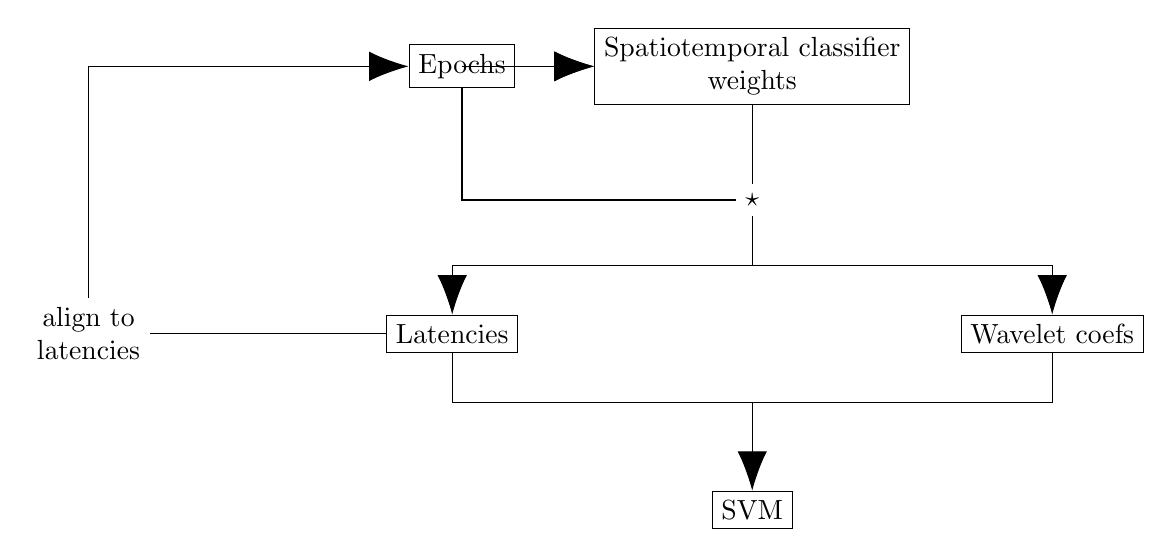
\begin{tikzpicture}
				\node[draw,align=center](class){Spatiotemporal classifier \\ weights};
				\node[below=of class,align=center](xcorr) {$\star$};
				\node[below=.5of xcorr](a1){};
				\node[draw,below=.5 of a1,align=center, xshift=-1.5in](latency) {Latencies};
				\node[draw,below=.5 of a1,align=center,xshift=1.5in](wav) {Wavelet coefs};
				\node[draw,left=of class,align=center](epochs) {Epochs};
				\node[left=3 of latency, align=center](align){align to \\ latencies};
				\node[below=.5of latency, xshift=1.5in](a2){};
				\node[draw, below= of a2,align=center](svm) {SVM};
				\node[left=.5of epochs](a3){};

				\draw[-{Latex[length=.2in]}] (epochs) to (class);
				\draw[-{Latex[length=5mm]}] (epochs) |- (class);
				\draw (class) to (xcorr);
				\draw (xcorr) to (a1.center);
				\draw[-{Latex[length=5mm]}] (a1.center) -| (latency);
				\draw[-{Latex[length=5mm]}] (a1.center) -| (wav);
				\draw (epochs) |- (xcorr);
				\draw (latency) |- (a2.center);
				\draw (wav) |- (a2.center);
				\draw[-{Latex[length=5mm]}] (a2.center)  to (svm);
				\draw (latency)  to (align);
				\draw (align.north)  |- (a3.center);
				\draw[-{Latex[length=5mm]}] (a3.center)  to (epochs);
			\end{tikzpicture}


		\end{tikzfigure}
		Visualization of convergence and alignment
	}

	\column{0.4}
	\block{Data collection}{
		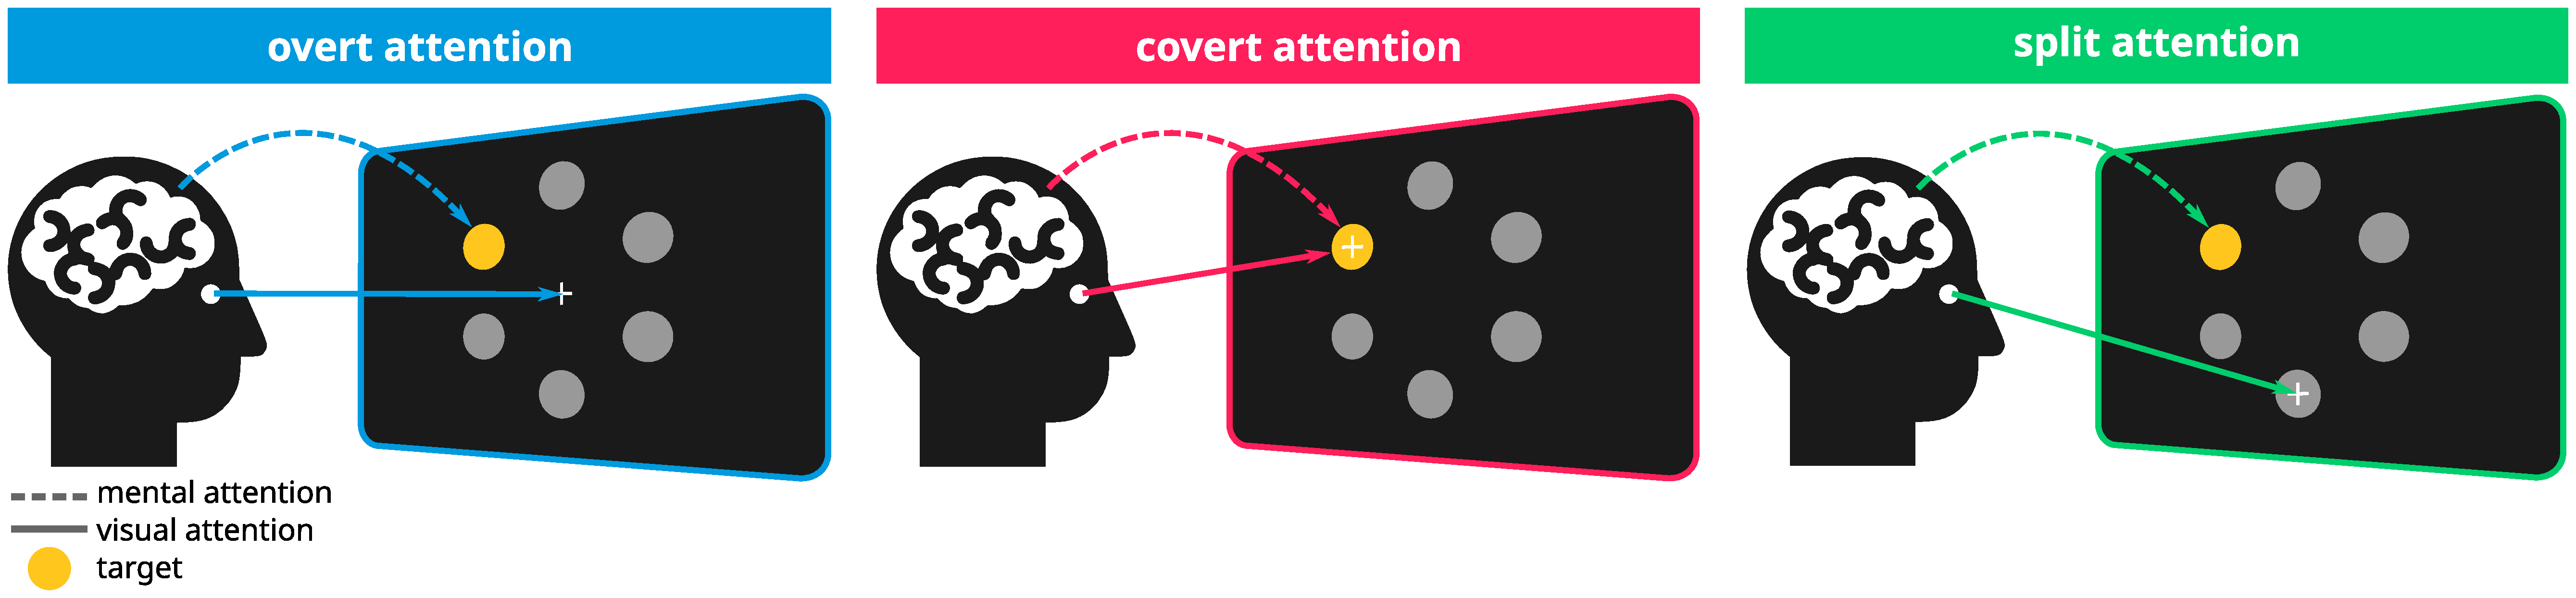
\includegraphics[width=\linewidth]{figures/attention_modes.eps}
	}
	\block{Results}{
		\begin{minipage}[c]{.25\linewidth}
			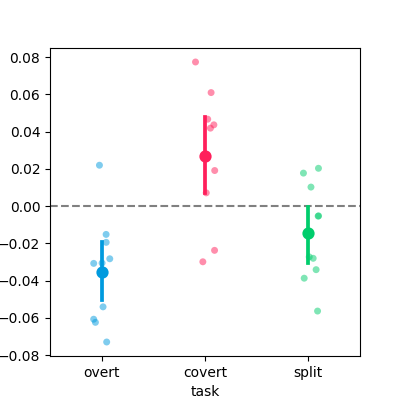
\includegraphics[width=\linewidth]{figures/classification_results_diff.png}
		\end{minipage}%
		\begin{minipage}[c]{.75\linewidth}
			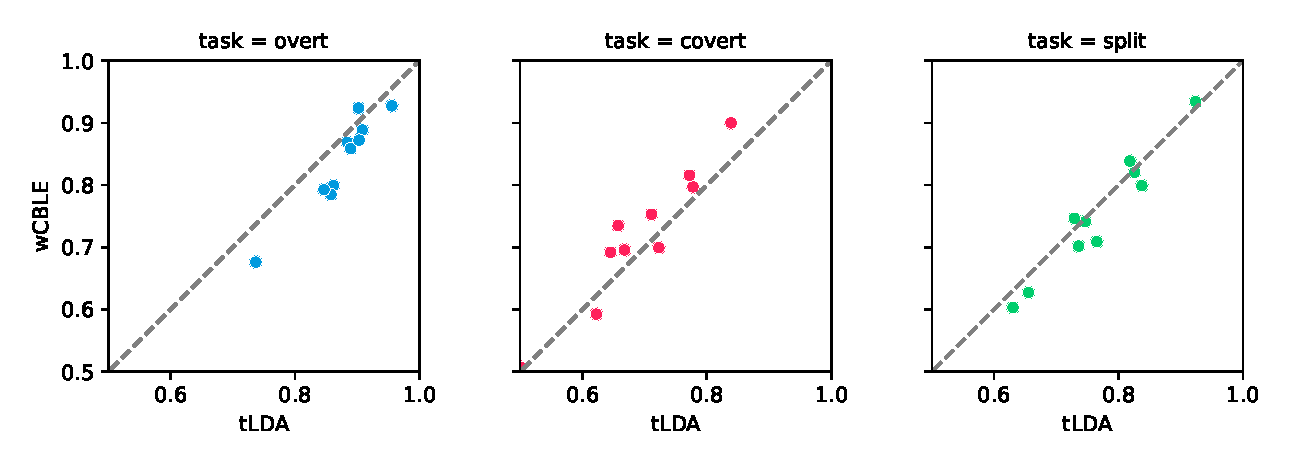
\includegraphics[width=\linewidth]{figures/classification_results_rel.eps}
		\end{minipage}%
		accuracy per repetition improvement
	}
	\block{References}{Text and more text}

\end{columns}

\end{document}
